\documentclass[aspectratio=169,11pt]{beamer}

\usepackage[T1]{fontenc}
\usepackage[utf8]{inputenc}
\usepackage[brazilian]{babel}
\usepackage{amsmath}
\usepackage{booktabs}
\usepackage{graphicx}
\usepackage{microtype}

\usetheme{Boadilla}

\definecolor{uftblue}{RGB}{0,67,101}
\definecolor{uftgreen}{RGB}{0,126,114}
\definecolor{lightgray}{RGB}{242,246,248}
\definecolor{alertred}{RGB}{166,44,44}

\setbeamercolor{structure}{fg=uftblue}
\setbeamercolor{frametitle}{fg=white,bg=uftblue}
\setbeamercolor{title}{fg=uftblue}
\setbeamercolor{subtitle}{fg=uftgreen}
\setbeamercolor{block title}{fg=white,bg=uftblue}
\setbeamercolor{block body}{fg=black,bg=lightgray}
\setbeamercolor{alerted text}{fg=alertred}
\setbeamercolor{author in head/foot}{fg=white,bg=uftblue}
\setbeamercolor{title in head/foot}{fg=white,bg=uftgreen}
\setbeamercolor{date in head/foot}{fg=white,bg=uftblue}

\setbeamertemplate{navigation symbols}{}
\setbeamertemplate{itemize item}{\color{uftgreen}$\blacktriangleright$}
\setbeamertemplate{itemize subitem}{\color{uftgreen}$\bullet$}
\setbeamerfont{title}{size=\Large,series=\bfseries}
\setbeamerfont{frametitle}{size=\large,series=\bfseries}
\setbeamerfont{footnote}{size=\tiny}

\newcommand{\fonte}[1]{%
  \vfill
  {\raggedright\tiny\color{gray}Fonte: #1\par}
}

\title[Ensino não presencial e SAEB]{Estratégias não presenciais e desempenho escolar na pandemia}
\subtitle{Uma análise municipal dos resultados do SAEB}
\author[Pedro Victor de Sá Castro]{Pedro Victor de Sá Castro}
\institute[UFT]{%
  Universidade Federal do Tocantins\\
  Curso de Ciências Econômicas\\[0.25em]
  Orientador: Prof. Marcleiton Ribeiro Morais
}
\date{Palmas -- TO, 2026}

\begin{document}

\begin{frame}[plain]
  \begin{columns}[c]
    \begin{column}{0.76\textwidth}
      \titlepage
    \end{column}
    \begin{column}{0.20\textwidth}
      \centering
      
\includegraphics[width=0.95\linewidth]{uft_logo.png}
    \end{column}
  \end{columns}
\end{frame}

\begin{frame}{Roteiro}
  \begin{enumerate}
    \item Contexto e problema de pesquisa
    \item Referencial teórico
    \item Dados e estratégia empírica
    \item Resultados
    \item Conclusão
  \end{enumerate}
\end{frame}

\section{Introdução}

\begin{frame}{Um choque na educação básica}
  \begin{columns}[T]
    \begin{column}{0.31\textwidth}
      \begin{block}{99,3\%}
        das escolas suspenderam atividades presenciais.
      \end{block}
    \end{column}
    \begin{column}{0.31\textwidth}
      \begin{block}{279 dias}
        foi o tempo médio de suspensão das aulas presenciais.
      \end{block}
    \end{column}
    \begin{column}{0.31\textwidth}
      \begin{block}{90,1\%}
        não retornaram às atividades presenciais em 2020.
      \end{block}
    \end{column}
  \end{columns}

  \vspace{0.8em}
  \begin{itemize}
    \item Mais de 98\% adotaram alguma estratégia não presencial.
    \item A capacidade de oferta variou entre redes e municípios.
    \item Adoção declarada não implica qualidade, duração ou alcance.
  \end{itemize}

  \fonte{Inep, pesquisa \textit{Resposta Educacional à Pandemia de Covid-19 no Brasil}.}
\end{frame}

\begin{frame}{Problema, objetivo e hipótese}
  \begin{block}{Pergunta de pesquisa}
    Municípios com baixa adoção de estratégias não presenciais apresentaram pior evolução no SAEB em 2021?
  \end{block}

  \begin{itemize}
    \item \textbf{Objetivo:} comparar a evolução da proficiência municipal em Língua Portuguesa e Matemática.
    \item \textbf{Grupo de interesse:} municípios com menos de 20\% das escolas declarando alguma estratégia não presencial.
    \item \textbf{Hipótese:} baixa adoção está associada a maior perda relativa de desempenho.
  \end{itemize}
\end{frame}

\section{Referencial teórico}

\begin{frame}{Educação, aprendizagem e capital humano}
  \begin{itemize}
    \item Educação é investimento que amplia capacidades produtivas e rendimentos.
    \item A aprendizagem representa a dimensão qualitativa do capital humano.
    \item A interrupção escolar reduz a acumulação de conhecimentos e habilidades.
    \item Desigualdades de conectividade e apoio familiar ampliam os efeitos do choque.
  \end{itemize}

  \vspace{0.8em}
  \begin{center}
    \large
    Interrupção escolar
    $\longrightarrow$ menor aprendizagem
    $\longrightarrow$ menor capital humano
  \end{center}

  \fonte{Schultz (1961), Becker (1975) e Mincer (1974).}
\end{frame}

\begin{frame}{Evidências relacionadas}
  \begin{itemize}
    \item \textbf{Fraga e Bacha (2013):} escolaridade e crescimento econômico estadual apresentam associação positiva.
    \item \textbf{Chaves et al. (2019):} resultados agregados não confirmam relação de longo prazo entre os indicadores analisados.
    \item \textbf{Bartholo et al. (2023):} perdas de aprendizagem e ampliação das desigualdades durante a pandemia.
    \item \textbf{Bof e Moraes (2022):} queda no desempenho do SAEB e diferenças entre grupos sociais.
  \end{itemize}

  \begin{block}{Lacuna explorada}
    Evidência municipal sobre a adoção de estratégias não presenciais e a evolução do desempenho escolar.
  \end{block}
\end{frame}

\section{Metodologia}

\begin{frame}{Base de dados}
  \begin{columns}[T]
    \begin{column}{0.48\textwidth}
      \textbf{Resposta educacional à pandemia}
      \begin{itemize}
        \item Censo Escolar 2020
        \item Informação por escola
        \item Agregação municipal
        \item Variável \texttt{PERC\_QUEST\_3\_S}
      \end{itemize}
    \end{column}
    \begin{column}{0.48\textwidth}
      \textbf{Sistema de Avaliação da Educação Básica}
      \begin{itemize}
        \item Edições de 2011 a 2023
        \item Médias do 5º e do 9º anos
        \item Língua Portuguesa
        \item Matemática
      \end{itemize}
    \end{column}
  \end{columns}

  \begin{block}{Unidade de análise}
    Painel de municípios por edição do SAEB.
  \end{block}

  \fonte{Inep; dados do SAEB obtidos por meio da Base dos Dados.}
\end{frame}

\begin{frame}{Definição do tratamento}
  \begin{block}{Municípios tratados}
    \[
      D_i = 1
      \quad\text{se}\quad
      \texttt{PERC\_QUEST\_3\_S} < 20\%
    \]
  \end{block}

  \begin{itemize}
    \item \textbf{58 municípios} formam o grupo de baixa adoção.
    \item Os demais municípios compõem o grupo de comparação.
    \item A variável mede a proporção de escolas que declarou adotar alguma estratégia.
    \item O indicador não observa intensidade, qualidade ou participação dos alunos.
  \end{itemize}
\end{frame}

\begin{frame}{Estratégia empírica}
  \begin{block}{Diferenças em diferenças}
    \[
      Y_{it} = \beta_0 + \beta_1 D_i + \beta_2 P_t
      + \beta_3(D_i \times P_t) + \varepsilon_{it}
    \]
  \end{block}

  \begin{itemize}
    \item $Y_{it}$: proficiência média do município $i$ no ano $t$.
    \item $P_t=1$ em 2021; $P_t=0$ nas demais edições.
    \item $\beta_3$: evolução relativa do grupo de baixa adoção em 2021.
    \item Erros-padrão agrupados por município.
  \end{itemize}

  \begin{alertblock}{Interpretação esperada}
    $\beta_3<0$: pior evolução relativa dos municípios com baixa adoção.
  \end{alertblock}
\end{frame}

\section{Resultados}

\begin{frame}{Trajetória da proficiência em Língua Portuguesa}
  \centering
  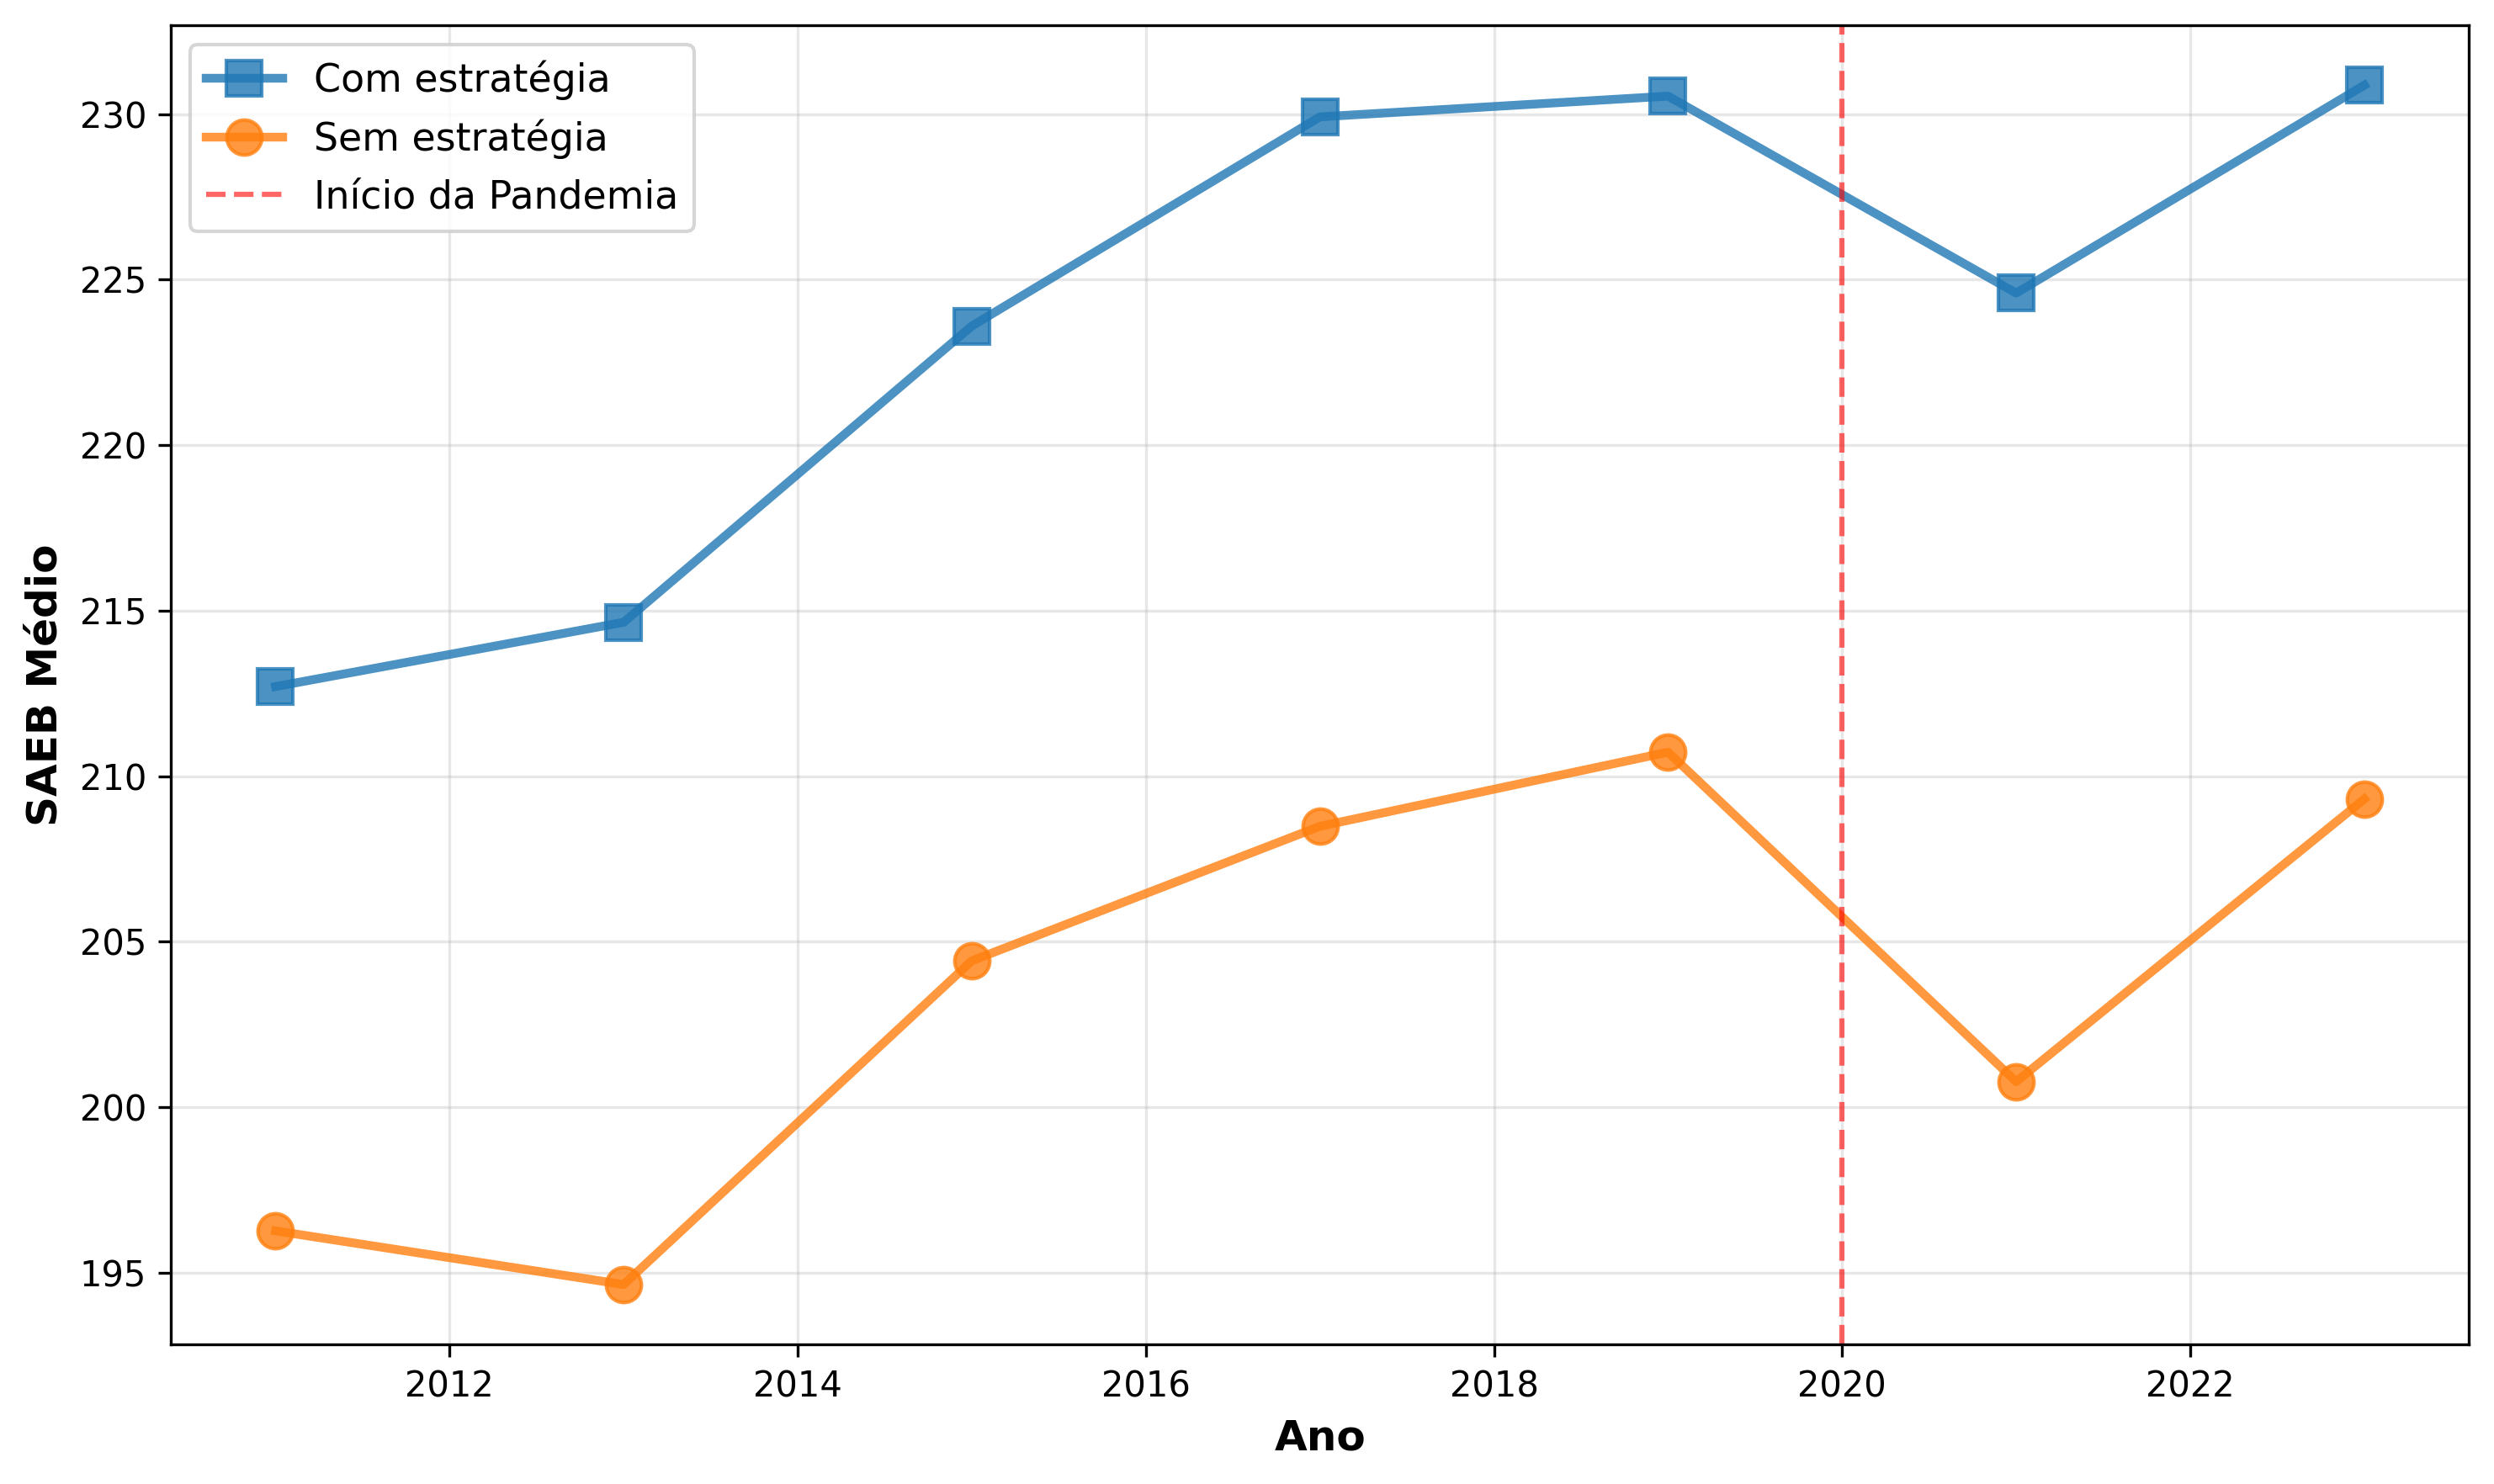
\includegraphics[height=0.72\textheight,keepaspectratio]{output/tendencias_paralelas_lp.png}

  \vspace{0.2em}
  \small O grupo de baixa adoção já apresentava desempenho inferior antes de 2021.
\end{frame}

\begin{frame}{Trajetória da proficiência em Matemática}
  \centering
  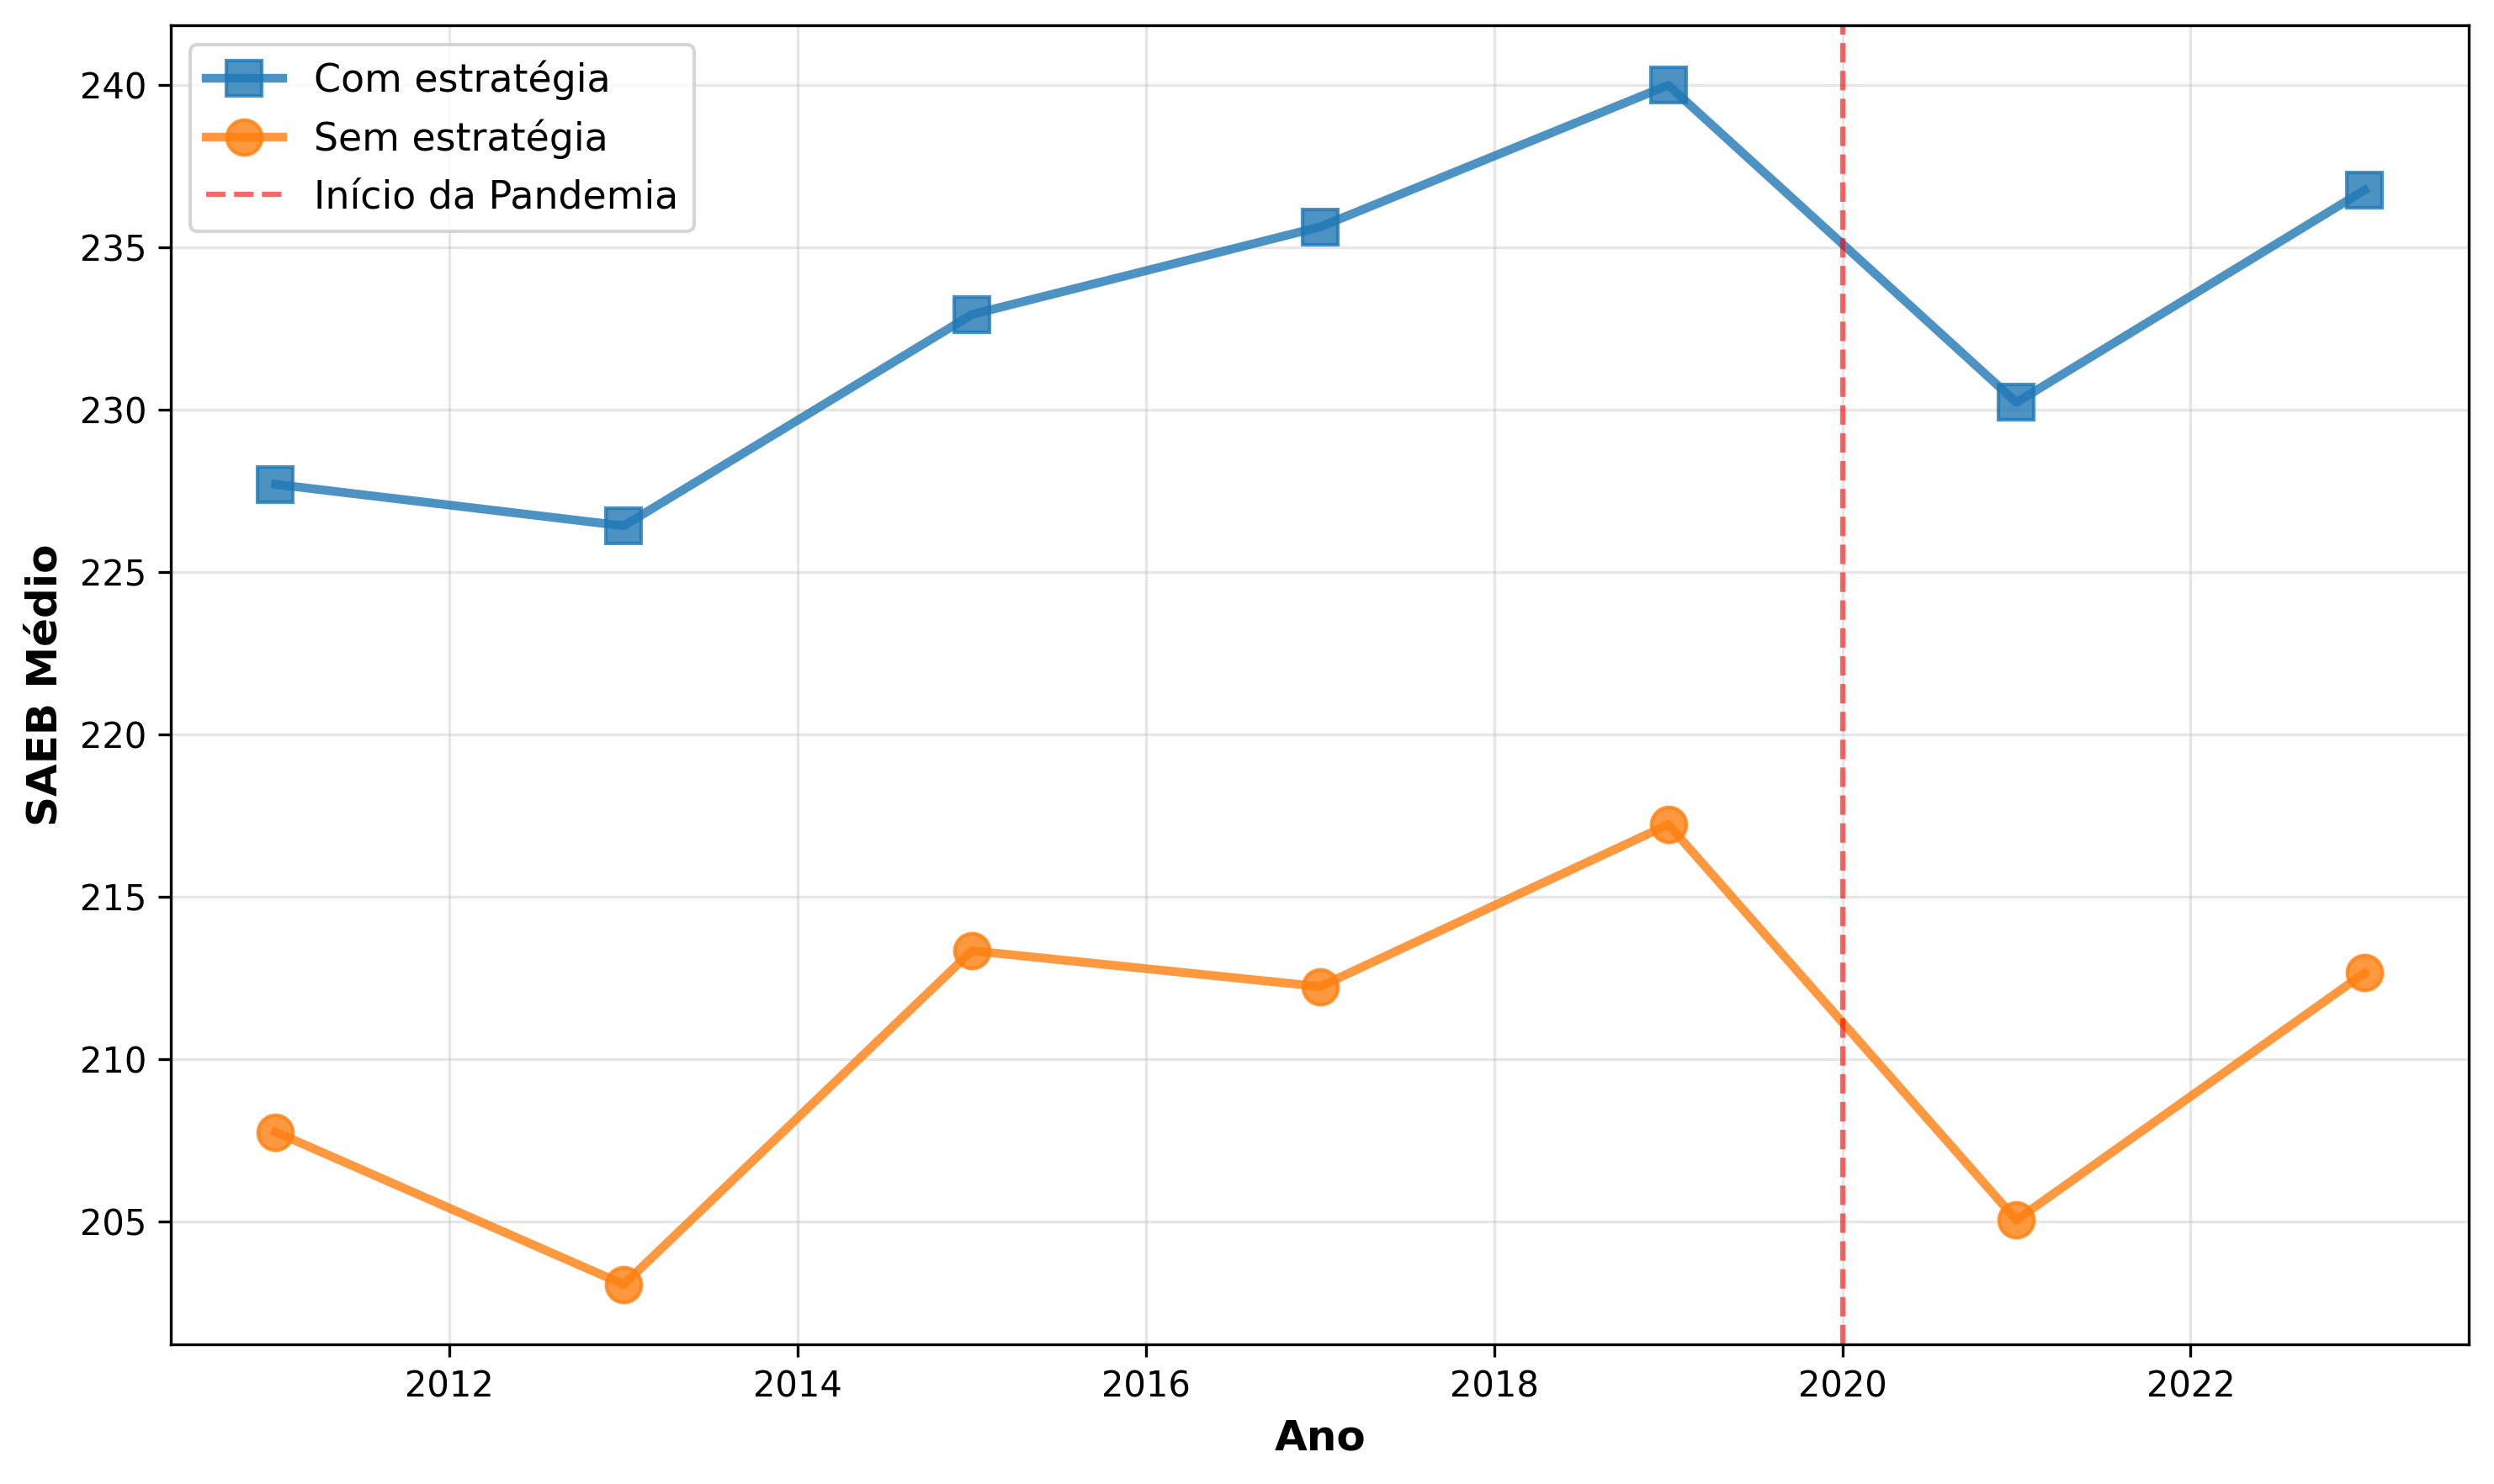
\includegraphics[height=0.72\textheight,keepaspectratio]{output/tendencias_paralelas_mt.png}

  \vspace{0.2em}
  \small A distância entre os grupos também é persistente em Matemática.
\end{frame}

\begin{frame}{Resultados do modelo de diferenças em diferenças}
  \centering
  \begin{tabular}{lrrrr}
    \toprule
    Disciplina & $\widehat{\beta}_3$ & Erro-padrão & Valor-$p$ & Significância \\
    \midrule
    Língua Portuguesa & $-4{,}06$ & $1{,}79$ & $0{,}023$ & 5\% \\
    Matemática        & $-2{,}97$ & $1{,}73$ & $0{,}085$ & 10\% \\
    \bottomrule
  \end{tabular}

  \vspace{1em}
  \begin{itemize}
    \item O grupo tratado teve evolução relativa menos favorável em 2021.
    \item A evidência é mais consistente para Língua Portuguesa.
    \item As diferenças anteriores eram de $-19{,}77$ e $-22{,}22$ pontos, respectivamente.
  \end{itemize}

  \fonte{Elaboração própria a partir dos dados do Inep.}
\end{frame}

\begin{frame}{Como interpretar os resultados}
  \begin{block}{Evidência encontrada}
    Baixa adoção está associada a uma evolução menos favorável da proficiência em 2021.
  \end{block}

  \begin{itemize}
    \item O resultado apoia parcialmente a hipótese do trabalho.
    \item Os grupos eram estruturalmente diferentes antes da pandemia.
    \item A adoção das estratégias não ocorreu de forma aleatória.
  \end{itemize}
\end{frame}

\begin{frame}{Limitações}
  \begin{itemize}
    \item Tratamento baseado em adoção declarada, sem medir qualidade ou alcance.
    \item Possível influência de conectividade, renda e capacidade administrativa.
    \item Médias agregadas entre anos escolares e redes de ensino.
    \item Apenas 2021 é definido como período posterior ao tratamento.
    \item Tendências prévias distintas entre os grupos.
  \end{itemize}
\end{frame}

\section{Conclusão}

\begin{frame}{Conclusão}
  \begin{itemize}
    \item Municípios com baixa adoção tiveram pior evolução relativa no SAEB de 2021.
    \item O efeito estimado foi maior e mais preciso em Língua Portuguesa.
    \item A hipótese recebeu apoio parcial, sem identificação causal forte.
    \item Preparação tecnológica e capacidade de resposta importam em crises educacionais.
  \end{itemize}

  \begin{block}{Implicações para políticas públicas}
    Conectividade, protocolos de ensino remoto e recuperação focalizada da aprendizagem.
  \end{block}
\end{frame}

\begin{frame}[plain]
  \begin{columns}[c]
    \begin{column}{0.76\textwidth}
      {\color{uftblue}\Huge\bfseries Obrigado!}\\[1.2em]
      {\Large Perguntas?}\\[2em]
      \textbf{Pedro Victor de Sá Castro}\\
      Curso de Ciências Econômicas -- UFT
    \end{column}
    \begin{column}{0.20\textwidth}
      \centering
      
\includegraphics[width=0.95\linewidth]{uft_logo.png}
    \end{column}
  \end{columns}
\end{frame}

\end{document}
